% psi(mu) = 1/|R(mu)| for the prior at 90 degrees with beta = 20: h0 = h3 = 10 sqrt 2; Newton from the left end
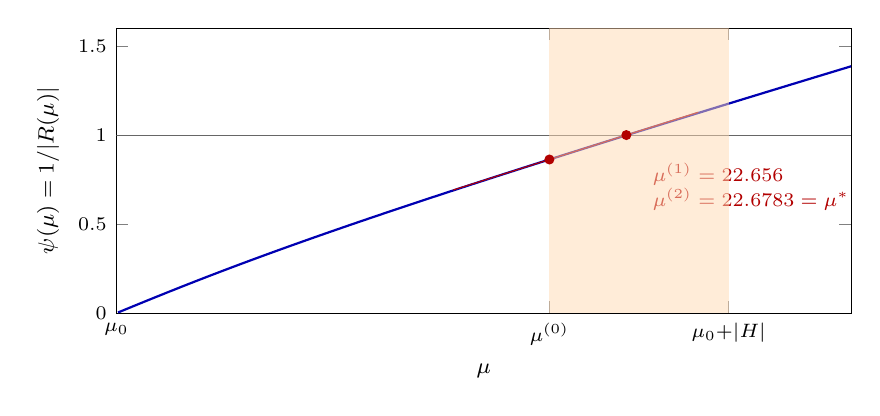
\begin{tikzpicture}
  \begin{axis}[width=0.9\textwidth, height=5.2cm, xmin=6, xmax=30, ymin=0, ymax=1.6,
      xlabel={$\mu$}, ylabel={$\psi(\mu) = 1 / |R(\mu)|$}, xtick={6,20.142,26}, xticklabels={$\mu_0$,$\mu^{(0)}$,$\mu_0{+}|H|$},
      tick label style={font=\scriptsize}, label style={font=\footnotesize}, samples=300]
    \addplot[thick, blue!70!black, domain=6.05:30] {1/sqrt(200/(x-6)^2 + 200/(x+4)^2)};
    \draw[black!60] (axis cs:6,1) -- (axis cs:30,1);
    % the tangent at mu(0) = 20.142 (psi = 0.86284, dpsi = 0.054555): it reaches 1 at 22.656
    \addplot[red!70!black, domain=17:25] {0.86284 + 0.054555*(x-20.14214)};
    \addplot[only marks, mark=*, mark size=1.6pt, red!70!black] coordinates {(20.14214,0.86284) (22.65593,1)};
    \draw[red!70!black, dashed] (axis cs:22.65593,1) -- (axis cs:22.65593,0.99895);
    \node[font=\scriptsize, red!70!black, anchor=north west, align=left] at (axis cs:23.2,0.9) {$\mu^{(1)} = 22.656$\\ $\mu^{(2)} = 22.6783 = \mu^*$};
    \fill[orange!30, opacity=0.5] (axis cs:20.142,0) rectangle (axis cs:26,1.6);
  \end{axis}
\end{tikzpicture}
